\section*{\shortstack[c]{CHAPTER 5. SIMULATION RESULTS AND PERFORMANCE\\[0.18cm]EVALUATION}}
\addcontentsline{toc}{section}{CHAPTER 5. SIMULATION RESULTS AND PERFORMANCE EVALUATION}

% =========================================================
% Numbering for Chapter 5
% =========================================================
\setcounter{section}{5}
\setcounter{subsection}{0}
\setcounter{subsubsection}{0}
\setcounter{figure}{0}
\setcounter{table}{0}
\setcounter{equation}{0}

\renewcommand{\thefigure}{5.\arabic{figure}}
\renewcommand{\thetable}{5.\arabic{table}}
\renewcommand{\theequation}{5.\arabic{equation}}
\renewcommand{\theHfigure}{5.\arabic{figure}}
\renewcommand{\theHtable}{5.\arabic{table}}
\renewcommand{\theHequation}{5.\arabic{equation}}

% =========================================================
% Chapter Introduction
% =========================================================
This chapter evaluates the baseline OFDM-LMMSE system, the baseline OTFS system, and the proposed OTFS-IM schemes under a common delay-Doppler channel simulation framework. The purpose is not only to compare final BER curves, but also to explain how index modulation changes the error structure of the receiver. Therefore, the results are organized from general BER comparison to equal-spectral-efficiency analysis, error decomposition, pattern-selection validation, and finally BER-SE trade-off across several \((n,k)\) configurations. This structure follows the design logic of Chapters 3 and 4 and is consistent with previous studies showing that OTFS detection and OTFS-IM performance depend jointly on channel sparsity, detector reliability, and activation-pattern design~\cite{Raviteja2018OTFSMP,Wu2024OTFSIMDetector,Liang2020OTFSIM}.

% =========================================================
% Chapter Sections
% =========================================================
% !TEX root = ../../main.tex

\subsection{Simulation Setup and Evaluation Metrics}

This section defines the simulation setting used to evaluate the baseline OFDM-LMMSE system, the baseline OTFS system, and the proposed OTFS-IM schemes. The purpose is to make the numerical results in the following sections reproducible and rate-aware. Since OTFS-IM changes both the signal structure and the number of information bits carried by each delay-Doppler block, the evaluation cannot rely only on BER curves. The simulation setup must also specify the spectral efficiency of each configuration and the error components associated with index modulation.

\subsubsection{Simulation Parameters}

All schemes are evaluated over the same delay-Doppler channel realization model and the same \(E_b/N_0\) range. The OTFS frame consists of \(N=10\) Doppler bins and \(M=12\) delay bins, resulting in \(NM=120\) resource elements per frame. The baseline OTFS and OFDM systems use 4-QAM modulation over all resource elements. The OTFS-IM system also uses 4-QAM on active positions, while additional information is conveyed by the activation pattern inside each IM block.

The channel is modeled as a discrete time-varying multipath channel with three propagation paths. The implemented delay taps are \([0,1,2]\), while the Doppler taps are randomly generated integer values in the simulated Doppler grid. Therefore, the simulation represents a Doppler-spread doubly selective channel rather than a channel tied to a specific physical velocity value. This choice is consistent with the purpose of the thesis: evaluating OTFS and OTFS-IM under delay-Doppler channel variations associated with high-mobility communication scenarios, without claiming a particular vehicular speed.

Table~\ref{tab:chapter5_simulation_parameters} summarizes the main simulation parameters used in the numerical evaluation.

\begin{table}[H]
    \centering
    \caption{Main simulation parameters}
    \label{tab:chapter5_simulation_parameters}
    \begin{tabularx}{\linewidth}{>{\RaggedRight\arraybackslash}p{4.4cm}
                                  >{\RaggedRight\arraybackslash}p{4.2cm}
                                  >{\RaggedRight\arraybackslash}X}
        \toprule
        Parameter & Value & Role in the simulation \\
        \midrule
        Doppler bins, \(N\) & 10 & Number of Doppler-domain grid points per OTFS frame \\
        \midrule
        Delay bins, \(M\) & 12 & Number of delay-domain grid points per OTFS frame \\
        \midrule
        Total resource elements & \(NM=120\) & Number of transmitted grid symbols per frame \\
        \midrule
        Baseline modulation & 4-QAM & Modulation used by OFDM-LMMSE and baseline OTFS \\
        \midrule
        Active-symbol modulation in OTFS-IM & 4-QAM & Modulation used on active IM positions \\
        \midrule
        Channel model & 3-tap delay-Doppler channel & Common channel model for OFDM, OTFS, and OTFS-IM \\
        \midrule
        Delay taps & \([0,1,2]\) & Discrete multipath delay positions \\
        \midrule
        Doppler taps & Random integer Doppler taps & Time variation and Doppler-spread behavior \\
        \midrule
        \(E_b/N_0\) range & \(0:5:20\) dB & SNR range used for BER curves \\
        \midrule
        OFDM-LMMSE frames & 1000 & Number of simulated OFDM frames per SNR point \\
        \midrule
        OTFS and OTFS-IM frames & 1000 & Number of simulated OTFS/OTFS-IM frames per SNR point \\
        \midrule
        Random-pattern diagnostic & 5 tables, 100 frames/table & Validation baseline for pattern-selection methods \\
        \bottomrule
    \end{tabularx}
\end{table}

The tested OTFS-IM configurations are selected to cover both equal-rate and reliability-oriented cases. Equal-rate configurations have the same spectral efficiency as the baseline OTFS system, while lower-rate configurations are included to show how reducing the number of transmitted bits per resource element can affect BER. For an IM block with \(n\) positions and \(k\) active positions, the number of index bits per block is
\begin{equation}
    b_1 = \left\lfloor \log_2 \binom{n}{k} \right\rfloor,
    \label{eq:chapter5_index_bits}
\end{equation}
and the number of active-symbol bits per block is
\begin{equation}
    b_2 = k \log_2 M_{\mathrm{QAM}}.
    \label{eq:chapter5_symbol_bits}
\end{equation}
Since 4-QAM is used in this thesis, \(\log_2 M_{\mathrm{QAM}}=2\). The spectral efficiency of the OTFS-IM mapping is then
\begin{equation}
    \eta_{\mathrm{IM}} = \frac{b_1+b_2}{n}.
    \label{eq:chapter5_im_spectral_efficiency}
\end{equation}

\begin{figure}[H]
    \centering
    \resizebox{0.98\linewidth}{!}{%
    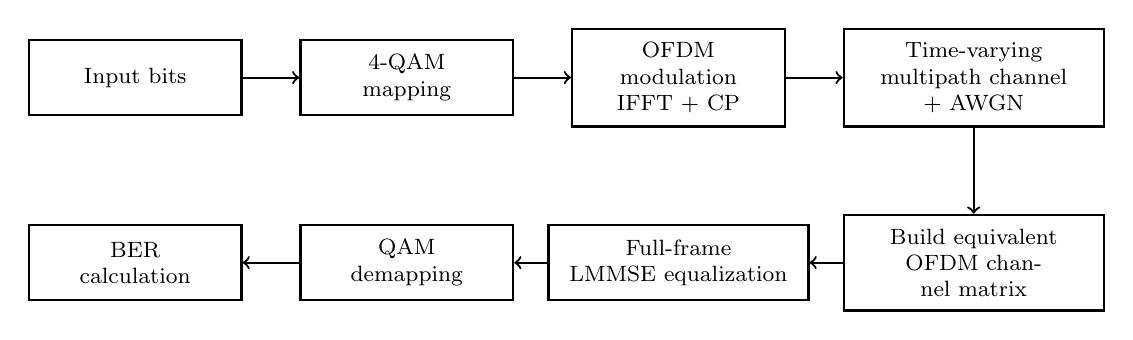
\begin{tikzpicture}[
        block/.style={
            rectangle,
            draw,
            thick,
            align=center,
            text width=2.35cm,
            minimum height=0.95cm,
            font=\footnotesize,
            inner sep=5pt
        },
        wideblock/.style={
            rectangle,
            draw,
            thick,
            align=center,
            text width=2.95cm,
            minimum height=0.95cm,
            font=\footnotesize,
            inner sep=5pt
        },
        arrow/.style={->, thick}
    ]
        \node[block] (bits) at (0,0) {Input bits};
        \node[block] (qam) at (3.45,0) {4-QAM\\mapping};
        \node[block] (ofdm) at (6.90,0) {OFDM\\modulation\\IFFT + CP};
        \node[wideblock] (chan) at (10.65,0) {Time-varying\\multipath channel\\+ AWGN};
        \node[wideblock] (hmat) at (10.65,-2.35) {Build equivalent\\OFDM channel matrix};
        \node[wideblock] (lmmse) at (6.90,-2.35) {Full-frame\\LMMSE equalization};
        \node[block] (demap) at (3.45,-2.35) {QAM\\demapping};
        \node[block] (ber) at (0,-2.35) {BER\\calculation};

        \draw[arrow] (bits.east) -- (qam.west);
        \draw[arrow] (qam.east) -- (ofdm.west);
        \draw[arrow] (ofdm.east) -- (chan.west);
        \draw[arrow] (chan.south) -- (hmat.north);
        \draw[arrow] (hmat.west) -- (lmmse.east);
        \draw[arrow] (lmmse.west) -- (demap.east);
        \draw[arrow] (demap.west) -- (ber.east);
    \end{tikzpicture}
    }
    \caption{OFDM-LMMSE baseline simulation flow}
    \label{fig:chapter5_ofdm_lmmse_flow}
\end{figure}

The OFDM-LMMSE flow in Fig.~\ref{fig:chapter5_ofdm_lmmse_flow} clarifies how the conventional multicarrier baseline is generated in the simulation. The receiver does not simply apply one-tap equalization; instead, it uses a full-frame LMMSE equalizer with channel knowledge. This makes the OFDM reference a stronger baseline for comparison with the delay-Doppler OTFS and OTFS-IM receivers.

Table~\ref{tab:chapter5_im_configurations} lists all simulated OTFS-IM configurations. The baseline OTFS and OFDM-LMMSE systems both have spectral efficiency \(2.00\) bits/symbol under 4-QAM transmission.

\begin{table}[H]
    \centering
    \caption{Simulated OTFS-IM configurations}
    \label{tab:chapter5_im_configurations}
    \begin{tabularx}{\linewidth}{>{\centering\arraybackslash}p{2.4cm}
                                  >{\centering\arraybackslash}p{1.4cm}
                                  >{\centering\arraybackslash}p{1.4cm}
                                  >{\centering\arraybackslash}p{1.4cm}
                                  >{\centering\arraybackslash}p{1.4cm}
                                  >{\centering\arraybackslash}p{2.4cm}
                                  >{\RaggedRight\arraybackslash}X}
        \toprule
        Configuration & \(n\) & \(k\) & \(b_1\) & \(b_2\) & \(\eta_{\mathrm{IM}}\) & Interpretation \\
        \midrule
        \(4\)-\(2\) & 4 & 2 & 2 & 4 & 1.50 & Lower-SE reliability-oriented case \\
        \midrule
        \(4\)-\(3\) & 4 & 3 & 2 & 6 & 2.00 & Equal-SE case \\
        \midrule
        \(5\)-\(3\) & 5 & 3 & 3 & 6 & 1.80 & Main pattern-selection validation case \\
        \midrule
        \(5\)-\(4\) & 5 & 4 & 2 & 8 & 2.00 & Equal-SE case \\
        \midrule
        \(6\)-\(3\) & 6 & 3 & 4 & 6 & 1.67 & Lower-SE reliability-oriented case \\
        \midrule
        \(6\)-\(4\) & 6 & 4 & 3 & 8 & 1.83 & Supplementary trade-off case \\
        \midrule
        \(6\)-\(5\) & 6 & 5 & 2 & 10 & 2.00 & Main larger-block equal-SE case \\
        \bottomrule
    \end{tabularx}
\end{table}

\subsubsection{Compared Schemes and Evaluation Metrics}

Four main schemes are compared in Chapter 5. The first one is OFDM-LMMSE, which is used as the conventional multicarrier reference. In the implementation, OFDM symbols are transmitted over the same time-varying channel as OTFS, and the receiver applies a full-frame LMMSE equalizer with perfect channel knowledge. Therefore, the OFDM curve should be understood as an equalized OFDM baseline, not as an unequalized OFDM receiver. This makes the comparison more meaningful because OTFS and OTFS-IM are not compared against an intentionally weak OFDM receiver.

The second scheme is the baseline OTFS system developed in Chapter 3. It uses full-grid 4-QAM mapping in the delay-Doppler domain and serves as the direct reference for evaluating whether OTFS-IM provides a useful improvement. The third scheme is OHD OTFS-IM, where the activation-pattern table is selected according to the optimized Hamming-distance criterion. The fourth scheme is B-OHD OTFS-IM, where the pattern-selection process additionally considers balance-related criteria such as carrier usage and closest-pair behavior. In configurations where OHD and B-OHD select effectively the same pattern set, their BER curves can overlap. This is not a simulation error; it means that the additional B-OHD criteria do not change the selected table for that specific \((n,k)\) setting.

Random pattern tables are also simulated as a diagnostic baseline. They are not treated as a proposed transmission method. Their role is to test whether deterministic pattern selection actually gives a meaningful advantage over arbitrary valid pattern choices. If a random table performs close to OHD or B-OHD in some SNR region, the result should be interpreted as evidence that pattern geometry alone is not always sufficient to determine the final BER.

The primary performance metric is the total bit error rate,
\begin{equation}
    \mathrm{BER} = \frac{N_{\mathrm{err}}}{N_{\mathrm{bits}}},
    \label{eq:chapter5_ber_definition}
\end{equation}
where \(N_{\mathrm{err}}\) is the number of incorrectly detected bits and \(N_{\mathrm{bits}}\) is the total number of transmitted information bits. For OTFS and OFDM, this BER directly measures the reliability of QAM symbol detection. For OTFS-IM, the total BER contains both index-bit errors and symbol-bit errors.

To explain the OTFS-IM behavior more clearly, the total BER is decomposed into index BER and symbol BER. Index BER measures the reliability of recovering the activation-pattern bits \(b_1\), while symbol BER measures the reliability of recovering the QAM bits \(b_2\) placed on active positions. In addition, the pattern error rate is reported as
\begin{equation}
    \mathrm{PER} = \frac{N_{\mathrm{wrong\ pattern}}}{N_{\mathrm{IM\ blocks}}},
    \label{eq:chapter5_pattern_error_rate}
\end{equation}
where \(N_{\mathrm{wrong\ pattern}}\) is the number of IM blocks in which the selected activation pattern is detected incorrectly. This metric is important because a wrong pattern decision can cause both index errors and symbol-placement errors.

Finally, spectral efficiency is used to distinguish equal-rate gains from rate-reliability trade-offs. A BER reduction is strongest when it is obtained at \(\eta_{\mathrm{IM}}=2.00\) bits/symbol, because this matches the spectral efficiency of the baseline OTFS system. If a configuration has lower BER but also lower spectral efficiency, the result is still useful, but it should be interpreted as a reliability-oriented trade-off rather than an unconditional improvement. For this reason, the final part of Chapter 5 presents both a configuration-level BER summary and a BER-SE trade-off plot across all simulated configurations.


% !TEX root = ../../main.tex

\subsection{Baseline BER Performance Comparison}

After defining the simulation setup, the first performance comparison is made between the conventional OFDM-LMMSE baseline, the baseline OTFS system, and the proposed OTFS-IM schemes. This comparison establishes the main BER trend before the detailed index-modulation analysis is presented. The representative configuration used in this section is \(n=6\), \(k=5\), because it has the same spectral efficiency as the baseline OTFS system:
\begin{equation}
    \eta_{\mathrm{IM}} = \eta_{\mathrm{OTFS}} = 2.00~\mathrm{bits/symbol}.
    \label{eq:chapter5_equal_se_65}
\end{equation}
Therefore, the BER comparison in this section is rate-fair. Any BER improvement of OTFS-IM over OTFS in this configuration is not obtained by reducing the number of transmitted bits per resource element.

\IfFileExists{Images/Chapter5/ber_overview_n6_k5.png}{%
\begin{figure}[H]
    \centering
    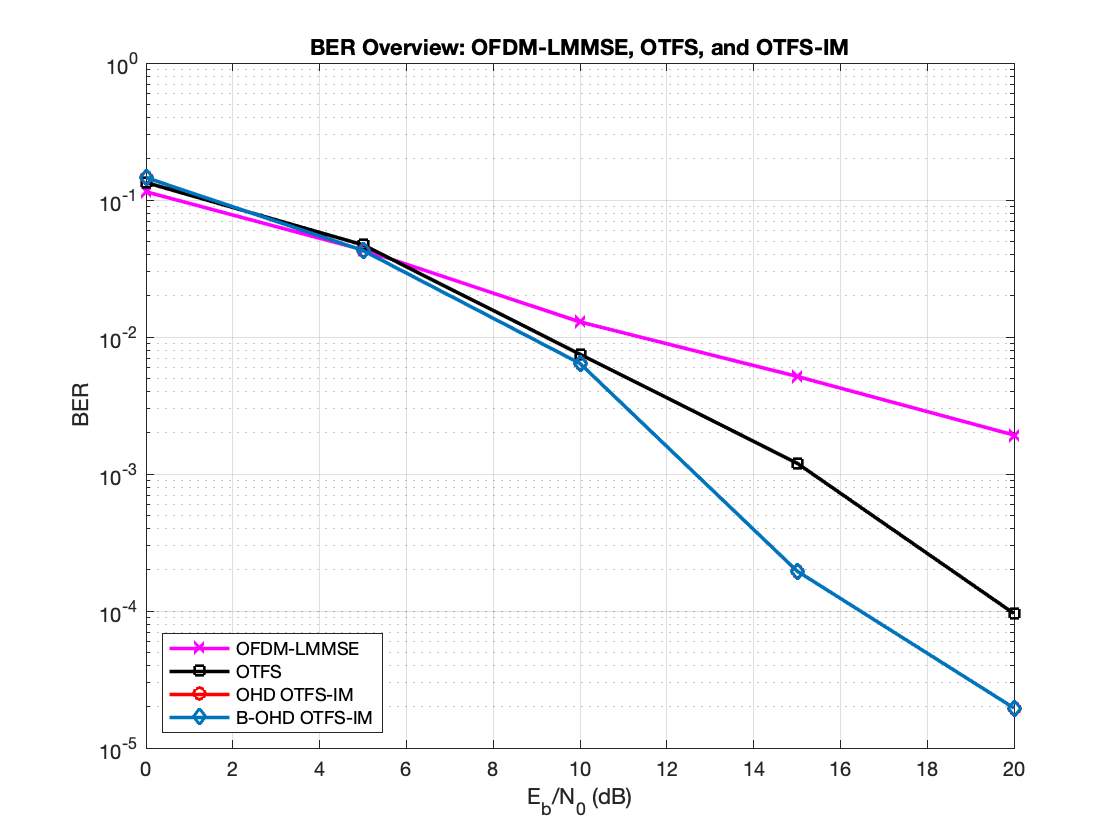
\includegraphics[width=0.88\linewidth]{Images/Chapter5/ber_overview_n6_k5.png}
    \caption{BER overview of OFDM-LMMSE, OTFS, and OTFS-IM for the \(n=6,k=5\) equal-SE configuration}
    \label{fig:chapter5_ber_overview_n6_k5}
\end{figure}
}{%
\begin{figure}[H]
    \centering
    \fbox{\begin{minipage}[c][5cm][c]{0.86\linewidth}
        \centering
        Required figure file is missing:\\
        Images/Chapter5/ber\_overview\_n6\_k5.png
    \end{minipage}}
    \caption{BER overview of OFDM-LMMSE, OTFS, and OTFS-IM for the \(n=6,k=5\) equal-SE configuration}
    \label{fig:chapter5_ber_overview_n6_k5}
\end{figure}
}

Figure~\ref{fig:chapter5_ber_overview_n6_k5} compares the BER of OFDM-LMMSE, baseline OTFS, OHD OTFS-IM, and B-OHD OTFS-IM over the simulated \(E_b/N_0\) range. The OFDM-LMMSE curve is included as the conventional multicarrier reference. Since it uses a full-frame LMMSE equalizer with perfect channel knowledge in the simulation, it should be interpreted as a meaningful OFDM benchmark rather than an unequalized OFDM receiver. The OTFS curve is the main delay-Doppler baseline, while the two OTFS-IM curves show the effect of adding index modulation and deterministic activation-pattern selection.

At low SNR, the BER of all schemes remains relatively high because the receiver is dominated by noise and uncertain symbol probabilities. In this region, the advantage of the delay-Doppler structure is not fully visible, and the additional index-detection task in OTFS-IM may even make the error behavior less stable. This can be observed around \(0\) dB, where the BER of OTFS-IM is not yet better than the baseline schemes. Such behavior is expected because the receiver must simultaneously detect both active positions and QAM symbols.

As the SNR increases, the benefit of OTFS and OTFS-IM becomes clearer. At \(10\) dB, the baseline OTFS BER is approximately \(7.49\times 10^{-3}\), while OHD OTFS-IM and B-OHD OTFS-IM both achieve approximately \(6.41\times 10^{-3}\) for the \(n=6,k=5\) configuration. This indicates a moderate but rate-fair improvement over baseline OTFS. The OFDM-LMMSE BER at the same SNR is approximately \(1.29\times 10^{-2}\), which is higher than the OTFS-based schemes under the same channel conditions.

The difference becomes more pronounced at higher SNR. At \(15\) dB, the baseline OTFS BER is approximately \(1.20\times 10^{-3}\), while OHD and B-OHD OTFS-IM decrease to about \(2.00\times 10^{-4}\). This is the most important region for interpreting the BER overview, because the noise level is low enough for the activation-pattern structure to become useful, but the error rate is still high enough to compare the schemes meaningfully. At \(20\) dB, the OTFS-IM curves approach the Monte Carlo resolution limit of the simulation. Therefore, the \(20\) dB point should be used cautiously and not over-interpreted as an exact zero-error result.

Table~\ref{tab:chapter5_representative_ber_n6_k5} gives the numerical BER values for the representative equal-SE configuration. The table is included to support the visual trend in Figure~\ref{fig:chapter5_ber_overview_n6_k5} and to make the comparison easier to reference in the discussion.

\begin{table}[H]
    \centering
    \caption{Representative BER values for the \(n=6,k=5\) equal-SE configuration}
    \label{tab:chapter5_representative_ber_n6_k5}
    \begin{tabularx}{\linewidth}{>{\centering\arraybackslash}p{2.1cm}
                                  >{\centering\arraybackslash}p{3.0cm}
                                  >{\centering\arraybackslash}p{2.4cm}
                                  >{\centering\arraybackslash}p{2.6cm}
                                  >{\Centering\arraybackslash}X}
        \toprule
        \(E_b/N_0\) (dB) & OFDM-LMMSE BER & OTFS BER & OHD OTFS-IM BER & B-OHD OTFS-IM BER \\
        \midrule
        0  & \(1.1480\times10^{-1}\) & \(1.3407\times10^{-1}\) & \(1.4573\times10^{-1}\) & \(1.4573\times10^{-1}\) \\
        \midrule
        5  & \(4.3280\times10^{-2}\) & \(4.7030\times10^{-2}\) & \(4.2800\times10^{-2}\) & \(4.2800\times10^{-2}\) \\
        \midrule
        10 & \(1.2880\times10^{-2}\) & \(7.4900\times10^{-3}\) & \(6.4100\times10^{-3}\) & \(6.4100\times10^{-3}\) \\
        \midrule
        15 & \(5.1600\times10^{-3}\) & \(1.2000\times10^{-3}\) & \(2.0000\times10^{-4}\) & \(2.0000\times10^{-4}\) \\
        \midrule
        20 & \(1.9300\times10^{-3}\) & \(1.0000\times10^{-4}\) & \(0\) & \(0\) \\
        \bottomrule
    \end{tabularx}
\end{table}

The table also shows that OHD and B-OHD have identical BER values in this configuration. This happens because the selected activation-pattern tables are effectively the same for \(n=6,k=5\). Since the valid pattern space is highly constrained in this case, the additional balancing criteria of B-OHD do not change the final selected pattern set. This observation is important for the following sections: B-OHD should not be expected to outperform OHD in every configuration. Its value becomes clearer only when the pattern space is large enough for the balance criterion to alter the selected table.

To illustrate a configuration where OHD and B-OHD do not completely overlap, Figure~\ref{fig:chapter5_ber_overview_n5_k3} shows the BER overview for \(n=5,k=3\). Unlike the previous equal-SE case, this configuration has
\begin{equation}
    \eta_{\mathrm{IM}} = 1.80~\mathrm{bits/symbol},
    \label{eq:chapter5_se_53}
\end{equation}
which is lower than the baseline OTFS spectral efficiency. Therefore, the \(n=5,k=3\) result should be interpreted as a reliability-rate trade-off rather than a direct rate-fair improvement.

\IfFileExists{Images/Chapter5/ber_overview_n5_k3.png}{%
\begin{figure}[H]
    \centering
    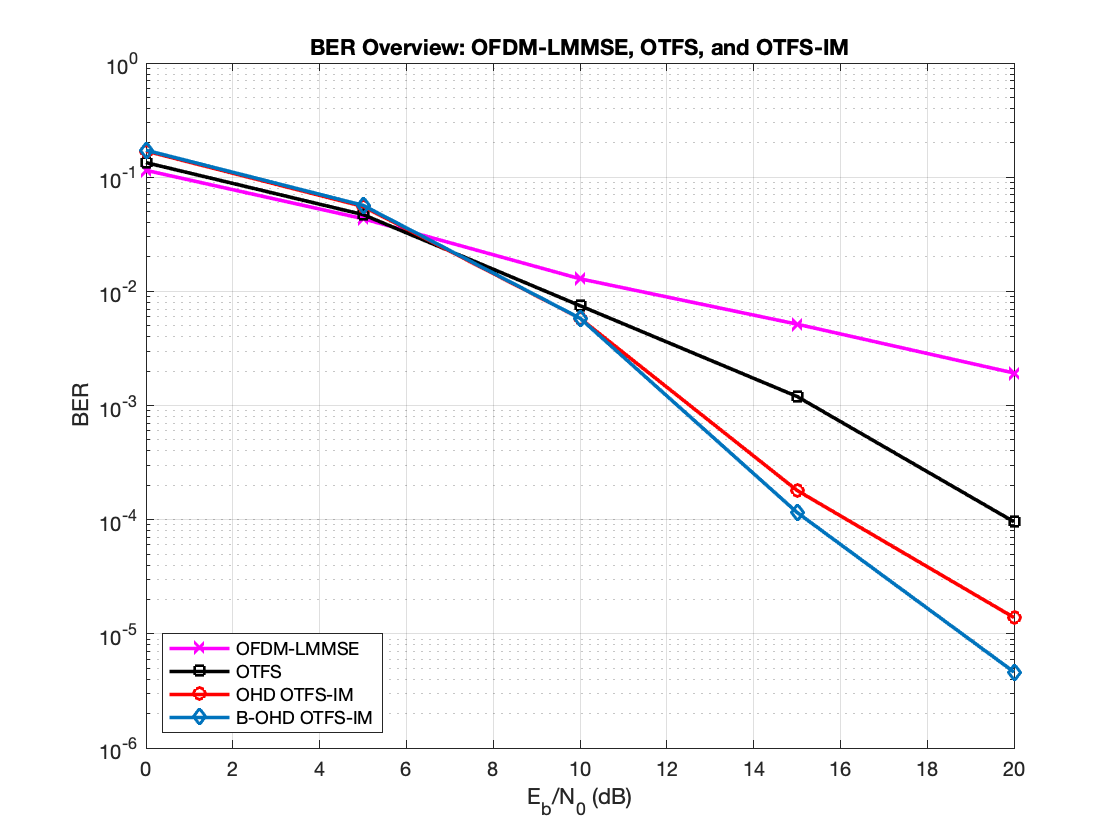
\includegraphics[width=0.88\linewidth]{Images/Chapter5/ber_overview_n5_k3.png}
    \caption{BER overview of OFDM-LMMSE, OTFS, and OTFS-IM for the \(n=5,k=3\) trade-off configuration}
    \label{fig:chapter5_ber_overview_n5_k3}
\end{figure}
}{%
\begin{figure}[H]
    \centering
    \fbox{\begin{minipage}[c][5cm][c]{0.86\linewidth}
        \centering
        Required figure file is missing:\\
        Images/Chapter5/ber\_overview\_n5\_k3.png
    \end{minipage}}
    \caption{BER overview of OFDM-LMMSE, OTFS, and OTFS-IM for the \(n=5,k=3\) trade-off configuration}
    \label{fig:chapter5_ber_overview_n5_k3}
\end{figure}
}

For \(n=5,k=3\), OHD and B-OHD no longer represent the same selected table. At \(10\) dB, both deterministic OTFS-IM schemes achieve approximately \(5.81\times10^{-3}\), which is lower than the baseline OTFS BER of approximately \(7.49\times10^{-3}\). At \(15\) dB, B-OHD becomes better than OHD, with a BER of about \(1.16\times10^{-4}\) compared with \(1.81\times10^{-4}\) for OHD. This behavior shows that the balancing criterion can change the high-SNR error trend, but the result must still be interpreted as a reliability-rate trade-off because \(\eta_{\mathrm{IM}}<\eta_{\mathrm{OTFS}}\). This configuration is therefore useful for pattern-selection analysis, while the \(n=6,k=5\) case remains the main rate-fair BER evidence.

Overall, this baseline comparison shows three important trends. First, OTFS-based transmission becomes more reliable than OFDM-LMMSE as the SNR increases under the considered delay-Doppler channel. Second, OTFS-IM can improve BER over baseline OTFS while maintaining the same spectral efficiency in the representative \(n=6,k=5\) case. Third, when the pattern table changes as in \(n=5,k=3\), OHD and B-OHD can produce different BER behavior, but the result must be interpreted together with spectral efficiency. For this reason, the next section focuses specifically on equal-spectral-efficiency OTFS-IM configurations before moving to pattern-level error analysis.


% !TEX root = ../../main.tex

\subsection{Equal Spectral Efficiency OTFS-IM Results}

The most important OTFS-IM results are obtained from configurations whose spectral efficiency is equal to that of the baseline OTFS system. In these cases, the comparison is not biased by a lower transmission rate. From Table~\ref{tab:chapter5_im_configurations}, the equal-SE configurations are \(n=4,k=3\), \(n=5,k=4\), and \(n=6,k=5\). All three cases satisfy
\begin{equation}
    \eta_{\mathrm{IM}} = 2.00~\mathrm{bits/symbol}
    =
    \eta_{\mathrm{OTFS}}.
    \label{eq:chapter5_equal_se_condition}
\end{equation}
Therefore, these configurations are used to evaluate whether OTFS-IM can improve the BER performance without sacrificing spectral efficiency.

Table~\ref{tab:chapter5_equal_se_ber_summary} summarizes the BER values of the equal-SE configurations at \(10\) dB and \(15\) dB. These two SNR points are more informative than the extreme high-SNR point because they avoid over-interpreting zero-error or near-zero-error outcomes caused by finite Monte Carlo simulation length.

\begin{table}[H]
    \centering
    \caption{BER summary of equal-SE OTFS-IM configurations}
    \label{tab:chapter5_equal_se_ber_summary}
    \begin{tabularx}{\linewidth}{>{\centering\arraybackslash}p{2.4cm}
                                  >{\centering\arraybackslash}p{1.6cm}
                                  >{\centering\arraybackslash}p{2.0cm}
                                  >{\centering\arraybackslash}p{2.2cm}
                                  >{\centering\arraybackslash}p{2.2cm}
                                  >{\Centering\arraybackslash}X}
        \toprule
        Configuration & \(E_b/N_0\) & OTFS BER & OHD OTFS-IM BER & B-OHD OTFS-IM BER & Interpretation \\
        \midrule
        \(4\)-\(3\) & 10 dB & \(7.49\times10^{-3}\) & \(6.71\times10^{-3}\) & \(6.71\times10^{-3}\) & Slight rate-fair gain \\
        \midrule
        \(4\)-\(3\) & 15 dB & \(1.20\times10^{-3}\) & \(2.20\times10^{-4}\) & \(2.20\times10^{-4}\) & Clear high-SNR gain \\
        \midrule
        \(5\)-\(4\) & 10 dB & \(7.49\times10^{-3}\) & \(6.64\times10^{-3}\) & \(6.64\times10^{-3}\) & Slight rate-fair gain \\
        \midrule
        \(5\)-\(4\) & 15 dB & \(1.20\times10^{-3}\) & \(3.20\times10^{-4}\) & \(3.20\times10^{-4}\) & Clear high-SNR gain \\
        \midrule
        \(6\)-\(5\) & 10 dB & \(7.49\times10^{-3}\) & \(6.41\times10^{-3}\) & \(6.41\times10^{-3}\) & Best 10 dB equal-SE case \\
        \midrule
        \(6\)-\(5\) & 15 dB & \(1.20\times10^{-3}\) & \(2.00\times10^{-4}\) & \(2.00\times10^{-4}\) & Strong equal-SE gain \\
        \bottomrule
    \end{tabularx}
\end{table}

The table shows a consistent trend. At \(10\) dB, all equal-SE OTFS-IM configurations improve slightly over baseline OTFS. The improvement is moderate because the receiver still needs to estimate both the active pattern and the active QAM symbols. At \(15\) dB, the improvement becomes more visible. In this SNR region, the noise level is low enough for the activation-pattern structure to contribute to more reliable detection.

Among the equal-SE configurations, \(n=6,k=5\) gives the best BER at both \(10\) dB and \(15\) dB in the deterministic OHD/B-OHD comparison. This is why it is used as the representative equal-SE case in Figure~\ref{fig:chapter5_ber_zoom_n6_k5}. The figure zooms into the \(5\)-\(20\) dB region and compares baseline OTFS with OHD and B-OHD OTFS-IM.

\IfFileExists{Images/Chapter5/ber_zoom_n6_k5.png}{%
\begin{figure}[H]
    \centering
    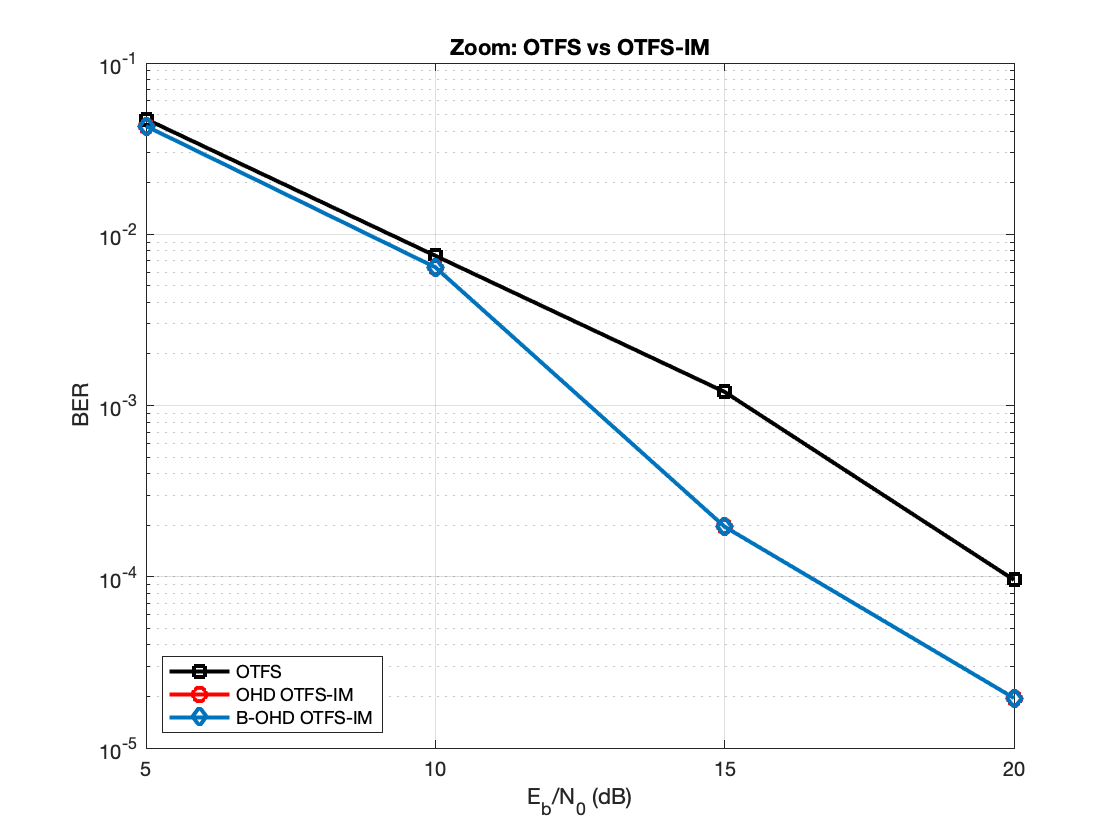
\includegraphics[width=0.88\linewidth]{Images/Chapter5/ber_zoom_n6_k5.png}
    \caption{BER zoom of baseline OTFS and equal-SE OTFS-IM for the \(n=6,k=5\) configuration}
    \label{fig:chapter5_ber_zoom_n6_k5}
\end{figure}
}{%
\begin{figure}[H]
    \centering
    \fbox{\begin{minipage}[c][5cm][c]{0.86\linewidth}
        \centering
        Required figure file is missing:\\
        Images/Chapter5/ber\_zoom\_n6\_k5.png
    \end{minipage}}
    \caption{BER zoom of baseline OTFS and equal-SE OTFS-IM for the \(n=6,k=5\) configuration}
    \label{fig:chapter5_ber_zoom_n6_k5}
\end{figure}
}

Figure~\ref{fig:chapter5_ber_zoom_n6_k5} confirms that the OTFS-IM curves become lower than the baseline OTFS curve from the medium-SNR region onward. At \(5\) dB, the schemes are close because detection is still noise-limited. At \(10\) dB and above, the index-modulated structure begins to provide a measurable BER reduction. Since the spectral efficiency is unchanged, this result is stronger than a lower-rate BER gain.

Another important observation is that OHD and B-OHD overlap in all three equal-SE configurations listed in Table~\ref{tab:chapter5_equal_se_ber_summary}. This does not indicate a plotting error. For \(n=4,k=3\), the number of valid activation patterns is \(\binom{4}{3}=4\), and the number of index-addressable patterns is also four. Therefore, all valid patterns are selected, leaving no additional freedom for B-OHD to improve the table. For \(n=5,k=4\) and \(n=6,k=5\), the valid pattern sets are also highly constrained, so the OHD and B-OHD selection criteria lead to the same effective pattern table.

This result clarifies the role of B-OHD in the thesis. B-OHD is not expected to improve every configuration. Its advantage can only appear when there is enough freedom to choose among multiple candidate pattern sets with the same minimum Hamming distance. In equal-SE configurations with a small or constrained pattern space, OHD and B-OHD may naturally become identical. This is why the \(n=5,k=3\) configuration is later used for pattern-selection validation, while the equal-SE configurations are used mainly to prove that OTFS-IM can improve BER without reducing spectral efficiency.

In summary, the equal-SE results provide the most important evidence for the usefulness of OTFS-IM in this thesis. Across \(4\)-\(3\), \(5\)-\(4\), and \(6\)-\(5\), OTFS-IM maintains the same spectral efficiency as baseline OTFS and still obtains lower BER in the medium and high SNR regions. The improvement is not uniform at all SNR values, but the trend is consistent enough to justify a deeper error-decomposition analysis in the next section.


% !TEX root = ../../main.tex

\subsection{OTFS-IM Error Decomposition}

The BER curves in the previous sections show the final end-to-end performance of OTFS-IM. However, total BER alone does not explain where the errors are produced inside the index-modulated receiver. In OTFS-IM, a detected bit can be wrong because the receiver selects an incorrect active-position pattern, because it detects an incorrect QAM symbol on an active position, or because both events occur in the same IM block. Therefore, this section decomposes the OTFS-IM result into index BER, symbol BER, and pattern error rate.

The decomposition is especially useful for interpreting whether the performance of a pattern-selection method is limited by the geometry of the selected activation patterns or by the reliability of the symbol decisions after the active positions have already been estimated. In the simulation, the index BER is computed from the recovered pattern bits, the symbol BER is computed from the recovered QAM bits on the active positions, and the pattern error rate measures the probability that the active-position pattern of an IM block is detected incorrectly.

\IfFileExists{Images/Chapter5/error_decomposition_n6_k5.png}{%
\begin{figure}[H]
    \centering
    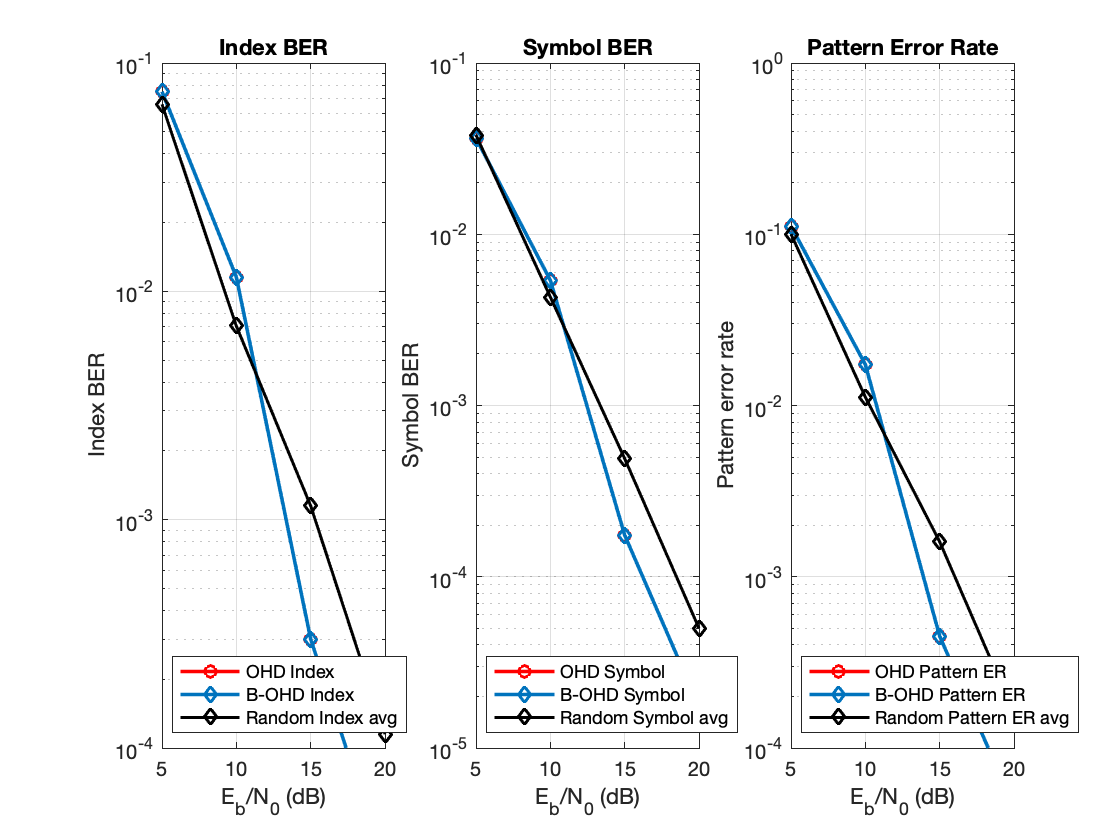
\includegraphics[width=0.95\linewidth]{Images/Chapter5/error_decomposition_n6_k5.png}
    \caption{Error decomposition of OHD and B-OHD OTFS-IM for \(n=6,k=5\)}
    \label{fig:chapter5_error_decomposition_n6_k5}
\end{figure}
}{%
\begin{figure}[H]
    \centering
    \fbox{%
        \begin{minipage}[c][0.25\textheight][c]{0.88\linewidth}
            \centering
            Required figure file is missing:\\
            Images/Chapter5/error\_decomposition\_n6\_k5.png
        \end{minipage}
    }
    \caption{Error decomposition of OHD and B-OHD OTFS-IM for \(n=6,k=5\)}
    \label{fig:chapter5_error_decomposition_n6_k5}
\end{figure}
}

Figure~\ref{fig:chapter5_error_decomposition_n6_k5} presents the error decomposition for the equal-spectral-efficiency configuration \(n=6,k=5\). This configuration is selected because it was used as the main equal-SE case in the previous section, where OTFS-IM and baseline OTFS both transmit \(2.00\) bits per resource element. As a result, the decomposition can be interpreted without the ambiguity of a rate advantage or a rate penalty.

At low SNR, both the index and symbol components are relatively large. This behavior is expected because the MP detector receives unreliable soft information from the delay-Doppler grid. Under this condition, the receiver may confuse the active positions and may also assign incorrect QAM symbols to positions that are detected as active. Therefore, the BER of OTFS-IM is not yet clearly separated into a purely index-limited or purely symbol-limited regime.

At medium SNR, the decomposition becomes more informative. For the \(n=6,k=5\) case, the OHD and B-OHD pattern tables are identical in the implemented simulation, so the two curves overlap. At \(E_b/N_0=10~\mathrm{dB}\), the total BER is approximately \(6.41\times10^{-3}\), while the measured index BER and symbol BER are approximately \(1.16\times10^{-2}\) and \(5.39\times10^{-3}\), respectively. In the bit-level contribution reported by the simulation, the symbol component accounts for about \(70\%\) of the total erroneous bits and the index component accounts for about \(30\%\). This means that, although pattern detection is important, the final BER is also strongly affected by the reliability of QAM symbol decisions on the detected active positions.

The pattern error rate provides a complementary view. At \(10~\mathrm{dB}\), the pattern error rate is approximately \(1.74\times10^{-2}\), which is higher than the total BER because one wrong pattern event is counted at the block level rather than at the bit level. A single pattern error does not necessarily imply that all bits in the IM block are wrong. Some symbol bits may still be recovered correctly, and some wrong active-position decisions may affect only part of the index-bit representation. For this reason, pattern error rate should not be compared directly with total BER as if they were the same metric. It is better interpreted as a diagnostic indicator of active-position reliability.

At higher SNR, the index and symbol components both decrease sharply. In the reported \(n=6,k=5\) result, the OTFS-IM BER approaches the Monte Carlo resolution at \(20~\mathrm{dB}\), and both index and symbol BER become nearly zero. This confirms that the detector is able to exploit the delay-Doppler representation effectively when the noise level is sufficiently low. It also shows that the performance gain observed in the BER curves is not produced by only one part of the receiver. Instead, it comes from the combined improvement in active-pattern detection and active-symbol detection.

The main conclusion from this decomposition is that OTFS-IM performance is jointly limited by pattern reliability and symbol reliability. Pattern selection can reduce the probability of confusing activation patterns, but it cannot fully determine the BER by itself. Once the active pattern is detected with reasonable reliability, the remaining errors are increasingly dominated by the QAM decisions on the active positions. This observation is important for the following section, where deterministic pattern selection is compared with random pattern selection. A good pattern table is beneficial, but its advantage is configuration-dependent and must be evaluated together with the detector behavior and the operating SNR range.


% !TEX root = ../../main.tex

\subsection{Pattern Selection Validation}

The previous sections evaluated OTFS-IM as an end-to-end transmission scheme. This section focuses on the pattern-selection component itself. In the proposed OTFS-IM transmitter, only a subset of all possible activation patterns is used for mapping the index bits. The purpose of OHD and B-OHD selection is to choose this subset more carefully than a purely arbitrary pattern table. The validation therefore compares deterministic pattern selection with a random-pattern diagnostic baseline.

The configuration \(n=5,k=3\) is used as the main validation case because it provides a non-trivial pattern-selection problem while keeping the exact OHD search feasible. For this configuration, there are \(\binom{5}{3}=10\) possible constant-weight activation patterns, and the system selects \(2^{b_1}=8\) patterns for index-bit mapping. Hence, OHD and B-OHD are forced to discard some candidate patterns, but the candidate set is still small enough to allow an exact comparison. This makes the configuration suitable for explaining the effect of pattern geometry without making the pattern-selection result visually or computationally excessive.

\IfFileExists{Images/Chapter5/pattern_geometry_n5_k3.png}{%
\begin{figure}[H]
    \centering
    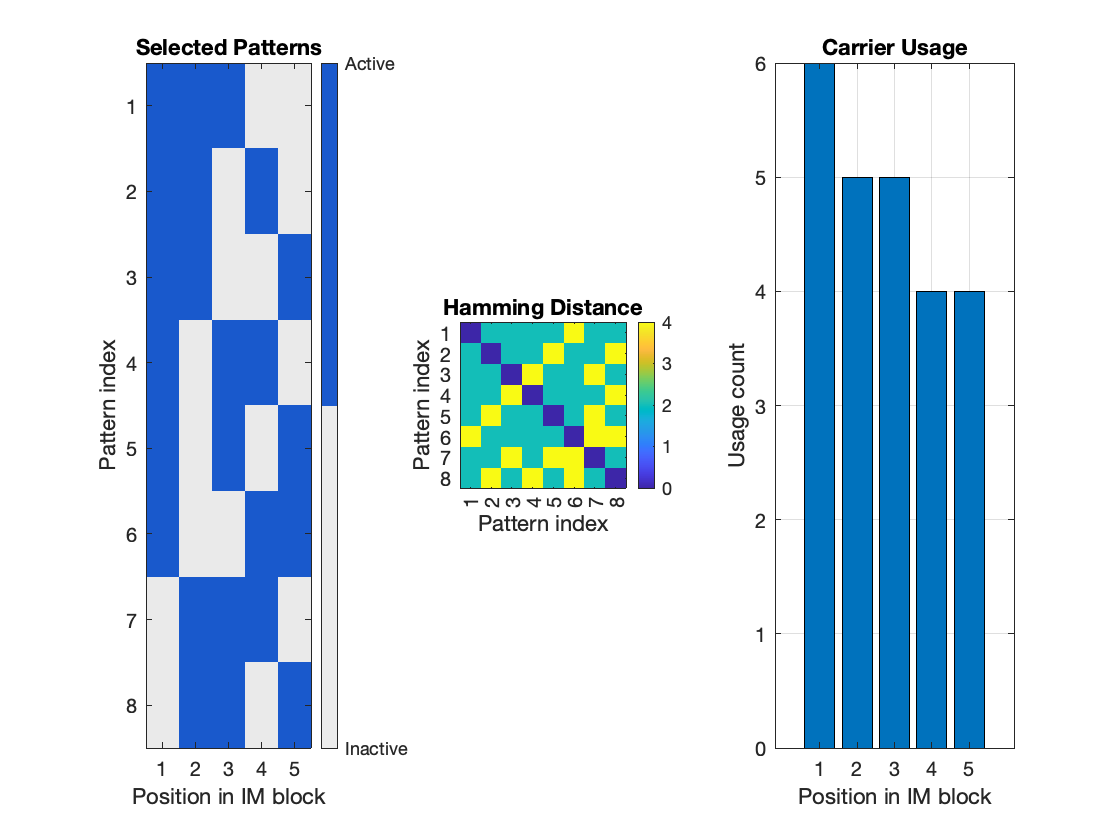
\includegraphics[width=0.92\linewidth]{Images/Chapter5/pattern_geometry_n5_k3.png}
    \caption{Selected pattern geometry for OHD-based OTFS-IM with \(n=5,k=3\)}
    \label{fig:chapter5_pattern_geometry_n5_k3}
\end{figure}
}{%
\begin{figure}[H]
    \centering
    \fbox{%
        \begin{minipage}[c][0.25\textheight][c]{0.88\linewidth}
            \centering
            Required figure file is missing:\\
            Images/Chapter5/pattern\_geometry\_n5\_k3.png
        \end{minipage}
    }
    \caption{Selected pattern geometry for OHD-based OTFS-IM with \(n=5,k=3\)}
    \label{fig:chapter5_pattern_geometry_n5_k3}
\end{figure}
}

Figure~\ref{fig:chapter5_pattern_geometry_n5_k3} illustrates the selected activation patterns and their geometric properties. The selected-pattern map shows which positions are active in each IM block. The Hamming-distance map indicates how different the selected patterns are from each other, while the carrier-usage plot shows whether the active positions are distributed evenly across the block. These three views are useful because pattern selection in OTFS-IM is not only about maximizing pairwise distance. A pattern table with good distance but unbalanced carrier usage may still create unequal position reliability.

For the \(n=5,k=3\) configuration, the spectral efficiency is
\begin{equation}
    \eta_{\mathrm{IM}}
    =
    \frac{\left\lfloor \log_2 \binom{5}{3} \right\rfloor + 3\log_2 4}{5}
    =
    \frac{3+6}{5}
    =
    1.80~\text{bits/symbol}.
    \label{eq:chapter5_se_53_validation}
\end{equation}
This rate is lower than the baseline OTFS rate of \(2.00~\text{bits/symbol}\), so this configuration should be interpreted as a reliability-oriented OTFS-IM setting rather than a strict equal-SE comparison. The BER improvement obtained in this case therefore represents a BER-SE trade-off: the system sacrifices \(10\%\) spectral efficiency to improve reliability in the medium-to-high-SNR region.

The geometry result also explains the difference between OHD and B-OHD. With OHD, the selected pattern table has carrier usage \([6,5,5,4,4]\), which indicates that the first position is activated more often than the last two positions. B-OHD preserves the same minimum Hamming distance but improves the usage balance to approximately \([5,4,5,5,5]\). This does not change the basic OTFS-IM structure, but it makes the selected pattern table less biased toward a small number of positions. Such balancing is expected to be more useful when the detector output is already reliable enough for the remaining pattern-geometry differences to matter.

\IfFileExists{Images/Chapter5/pattern_validation_n5_k3.png}{%
\begin{figure}[H]
    \centering
    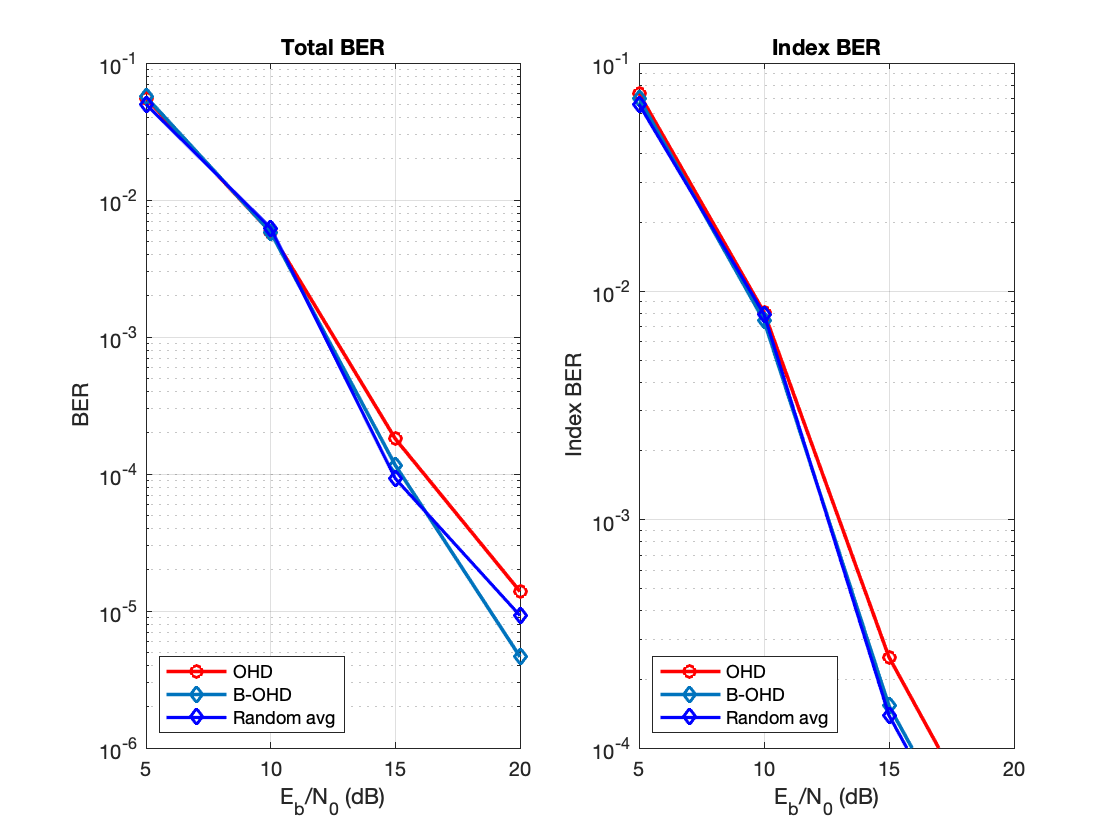
\includegraphics[width=0.95\linewidth]{Images/Chapter5/pattern_validation_n5_k3.png}
    \caption{Validation of OHD and B-OHD pattern selection against random pattern tables for \(n=5,k=3\)}
    \label{fig:chapter5_pattern_validation_n5_k3}
\end{figure}
}{%
\begin{figure}[H]
    \centering
    \fbox{%
        \begin{minipage}[c][0.28\textheight][c]{0.88\linewidth}
            \centering
            Required figure file is missing:\\
            Images/Chapter5/pattern\_validation\_n5\_k3.png
        \end{minipage}
    }
    \caption{Validation of OHD and B-OHD pattern selection against random pattern tables for \(n=5,k=3\)}
    \label{fig:chapter5_pattern_validation_n5_k3}
\end{figure}
}

Figure~\ref{fig:chapter5_pattern_validation_n5_k3} compares OHD, B-OHD, and the random-pattern average. The random curve is not used as a proposed design method in this thesis. Instead, it is used as a diagnostic reference to check whether the deterministic selection rules provide a meaningful advantage over arbitrary pattern choices. This comparison is necessary because a random pattern table can sometimes have favorable distance or usage properties, especially when the candidate set is small.

At \(10~\mathrm{dB}\), the total BER values are approximately \(5.81\times10^{-3}\), \(5.81\times10^{-3}\), and \(6.24\times10^{-3}\) for OHD, B-OHD, and random selection, respectively. At this SNR point, deterministic pattern selection provides a modest but visible improvement over the random average. The index BER values are also close: \(8.10\times10^{-3}\) for OHD, \(7.43\times10^{-3}\) for B-OHD, and \(7.94\times10^{-3}\) for the random average. This indicates that B-OHD slightly improves the index reliability compared with OHD while remaining competitive with the random baseline.

At \(15~\mathrm{dB}\), the performance difference becomes more visible in the total BER. OHD reaches approximately \(1.81\times10^{-4}\), B-OHD reaches \(1.16\times10^{-4}\), and the random average reaches \(9.0\times10^{-5}\). The random average is slightly lower at this point, but B-OHD still improves over the original OHD table. This result should not be interpreted as a failure of deterministic pattern selection. Rather, it shows that random pattern tables can occasionally be strong, and that the proposed deterministic design should be evaluated against them instead of only against the OTFS baseline.

The pattern error rate provides an additional explanation. At \(10~\mathrm{dB}\), the pattern error rates are approximately \(1.47\times10^{-2}\), \(1.36\times10^{-2}\), and \(1.49\times10^{-2}\) for OHD, B-OHD, and random selection, respectively. B-OHD gives the lowest pattern error rate in this region, which is consistent with its improved carrier-usage balance. At \(15~\mathrm{dB}\), all three methods have very small pattern error rates, and the remaining BER differences become sensitive to both symbol decisions and Monte Carlo variation.

Overall, the \(n=5,k=3\) validation gives a clearer pattern-selection story than configurations where OHD and B-OHD overlap. OHD provides a structured pattern table based on Hamming-distance separation, while B-OHD improves the balance of the selected table without changing the OTFS-IM receiver. The results show that B-OHD can improve OHD, especially in the medium-to-high-SNR region. At the same time, the random baseline remains important because it shows that pattern selection is configuration-dependent and that Hamming distance alone does not guarantee universal superiority. This observation motivates future channel-aware or detector-aware pattern selection methods, while still supporting the use of structured pattern design in the present OTFS-IM system.


% !TEX root = ../../main.tex

\subsection{BER-SE Trade-Off Across Configurations}

The previous sections examined representative OTFS-IM configurations in detail. This section combines the available simulation results into a configuration-level comparison. The purpose is not only to identify the lowest BER curve, but also to interpret each result together with its spectral efficiency. This distinction is important because an OTFS-IM configuration may improve BER by reducing the number of transmitted information bits per block, while another configuration may preserve the same spectral efficiency as the baseline OTFS system.

Two summary figures are used for this comparison. The first figure compares the BER values of different OTFS-IM configurations at selected SNR points. This view is useful for quickly identifying which configurations operate below the OTFS reference curve. The second figure places the same BER values against spectral efficiency. This view clarifies whether a BER improvement is obtained at equal spectral efficiency or by accepting a lower-rate transmission mode.

\IfFileExists{Images/Chapter5/configuration_ber_summary.png}{%
\begin{figure}[H]
    \centering
    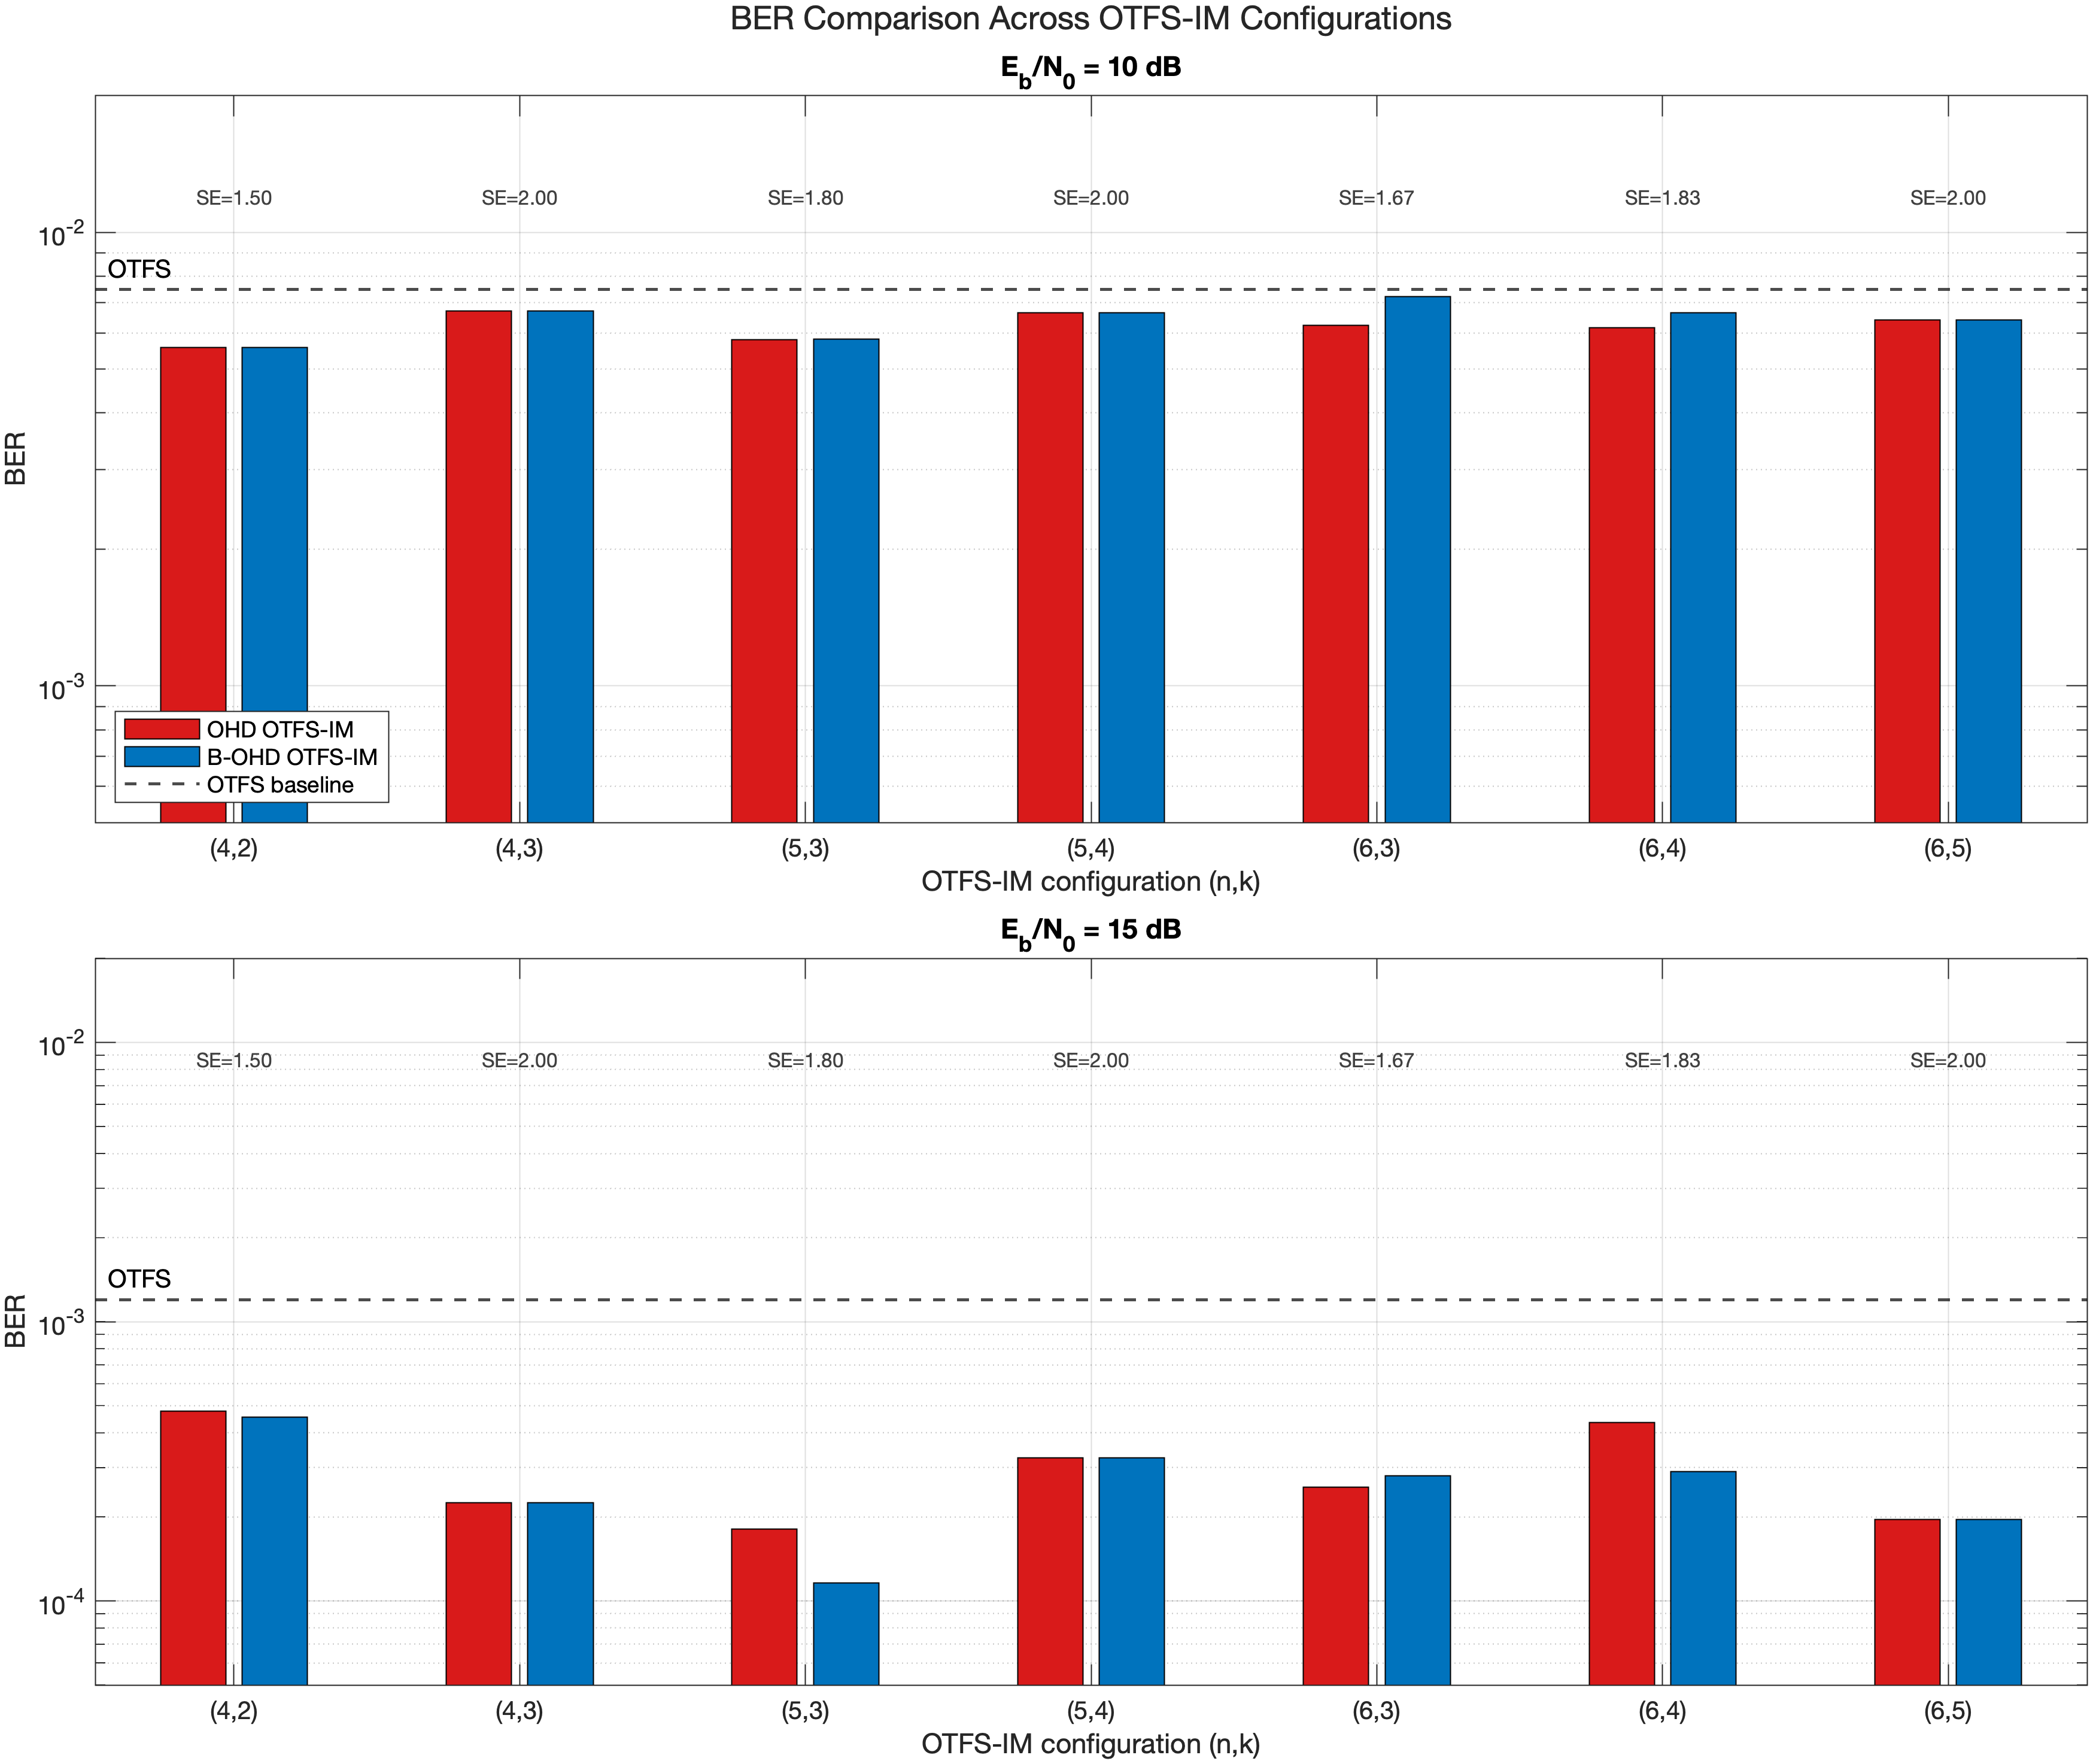
\includegraphics[width=0.95\linewidth]{Images/Chapter5/configuration_ber_summary.png}
    \caption{Configuration-level BER comparison for OHD and B-OHD OTFS-IM at selected SNR points}
    \label{fig:chapter5_configuration_ber_summary}
\end{figure}
}{%
\begin{figure}[H]
    \centering
    \fbox{%
        \begin{minipage}[c][0.28\textheight][c]{0.88\linewidth}
            \centering
            Required figure file is missing:\\
            Images/Chapter5/configuration\_ber\_summary.png
        \end{minipage}
    }
    \caption{Configuration-level BER comparison for OHD and B-OHD OTFS-IM at selected SNR points}
    \label{fig:chapter5_configuration_ber_summary}
\end{figure}
}

Figure~\ref{fig:chapter5_configuration_ber_summary} summarizes the BER of the simulated OTFS-IM configurations at \(E_b/N_0=10~\mathrm{dB}\) and \(E_b/N_0=15~\mathrm{dB}\). The dashed horizontal line represents the baseline OTFS BER at the same SNR value. Therefore, a bar below this line indicates that the corresponding OTFS-IM configuration achieves a lower BER than baseline OTFS at that operating point.

At \(10~\mathrm{dB}\), most OTFS-IM configurations are already below the OTFS baseline. However, the separation is moderate because the detector still operates in a region where both index errors and symbol errors contribute to the total BER. In this region, changing the pattern table from OHD to B-OHD does not always create a large visible gain. This behavior is consistent with the error-decomposition results: when the received reliability is still limited, the total BER is dominated not only by the geometric distance between activation patterns, but also by the quality of the MP detector output.

At \(15~\mathrm{dB}\), the difference between configurations becomes clearer. Several OTFS-IM configurations move further below the OTFS baseline, showing that index modulation can be beneficial in the medium-to-high-SNR region. The \(n=5,k=3\) case is particularly useful for pattern-selection validation because B-OHD improves over OHD while keeping the same IM block size and modulation order. This confirms that the balancing term in B-OHD can be meaningful when the selected pattern table is not identical to the OHD table. By contrast, in configurations such as \(n=6,k=5\), OHD and B-OHD may select effectively the same pattern table, so their BER curves overlap.

\IfFileExists{Images/Chapter5/ber_se_tradeoff.png}{%
\begin{figure}[H]
    \centering
    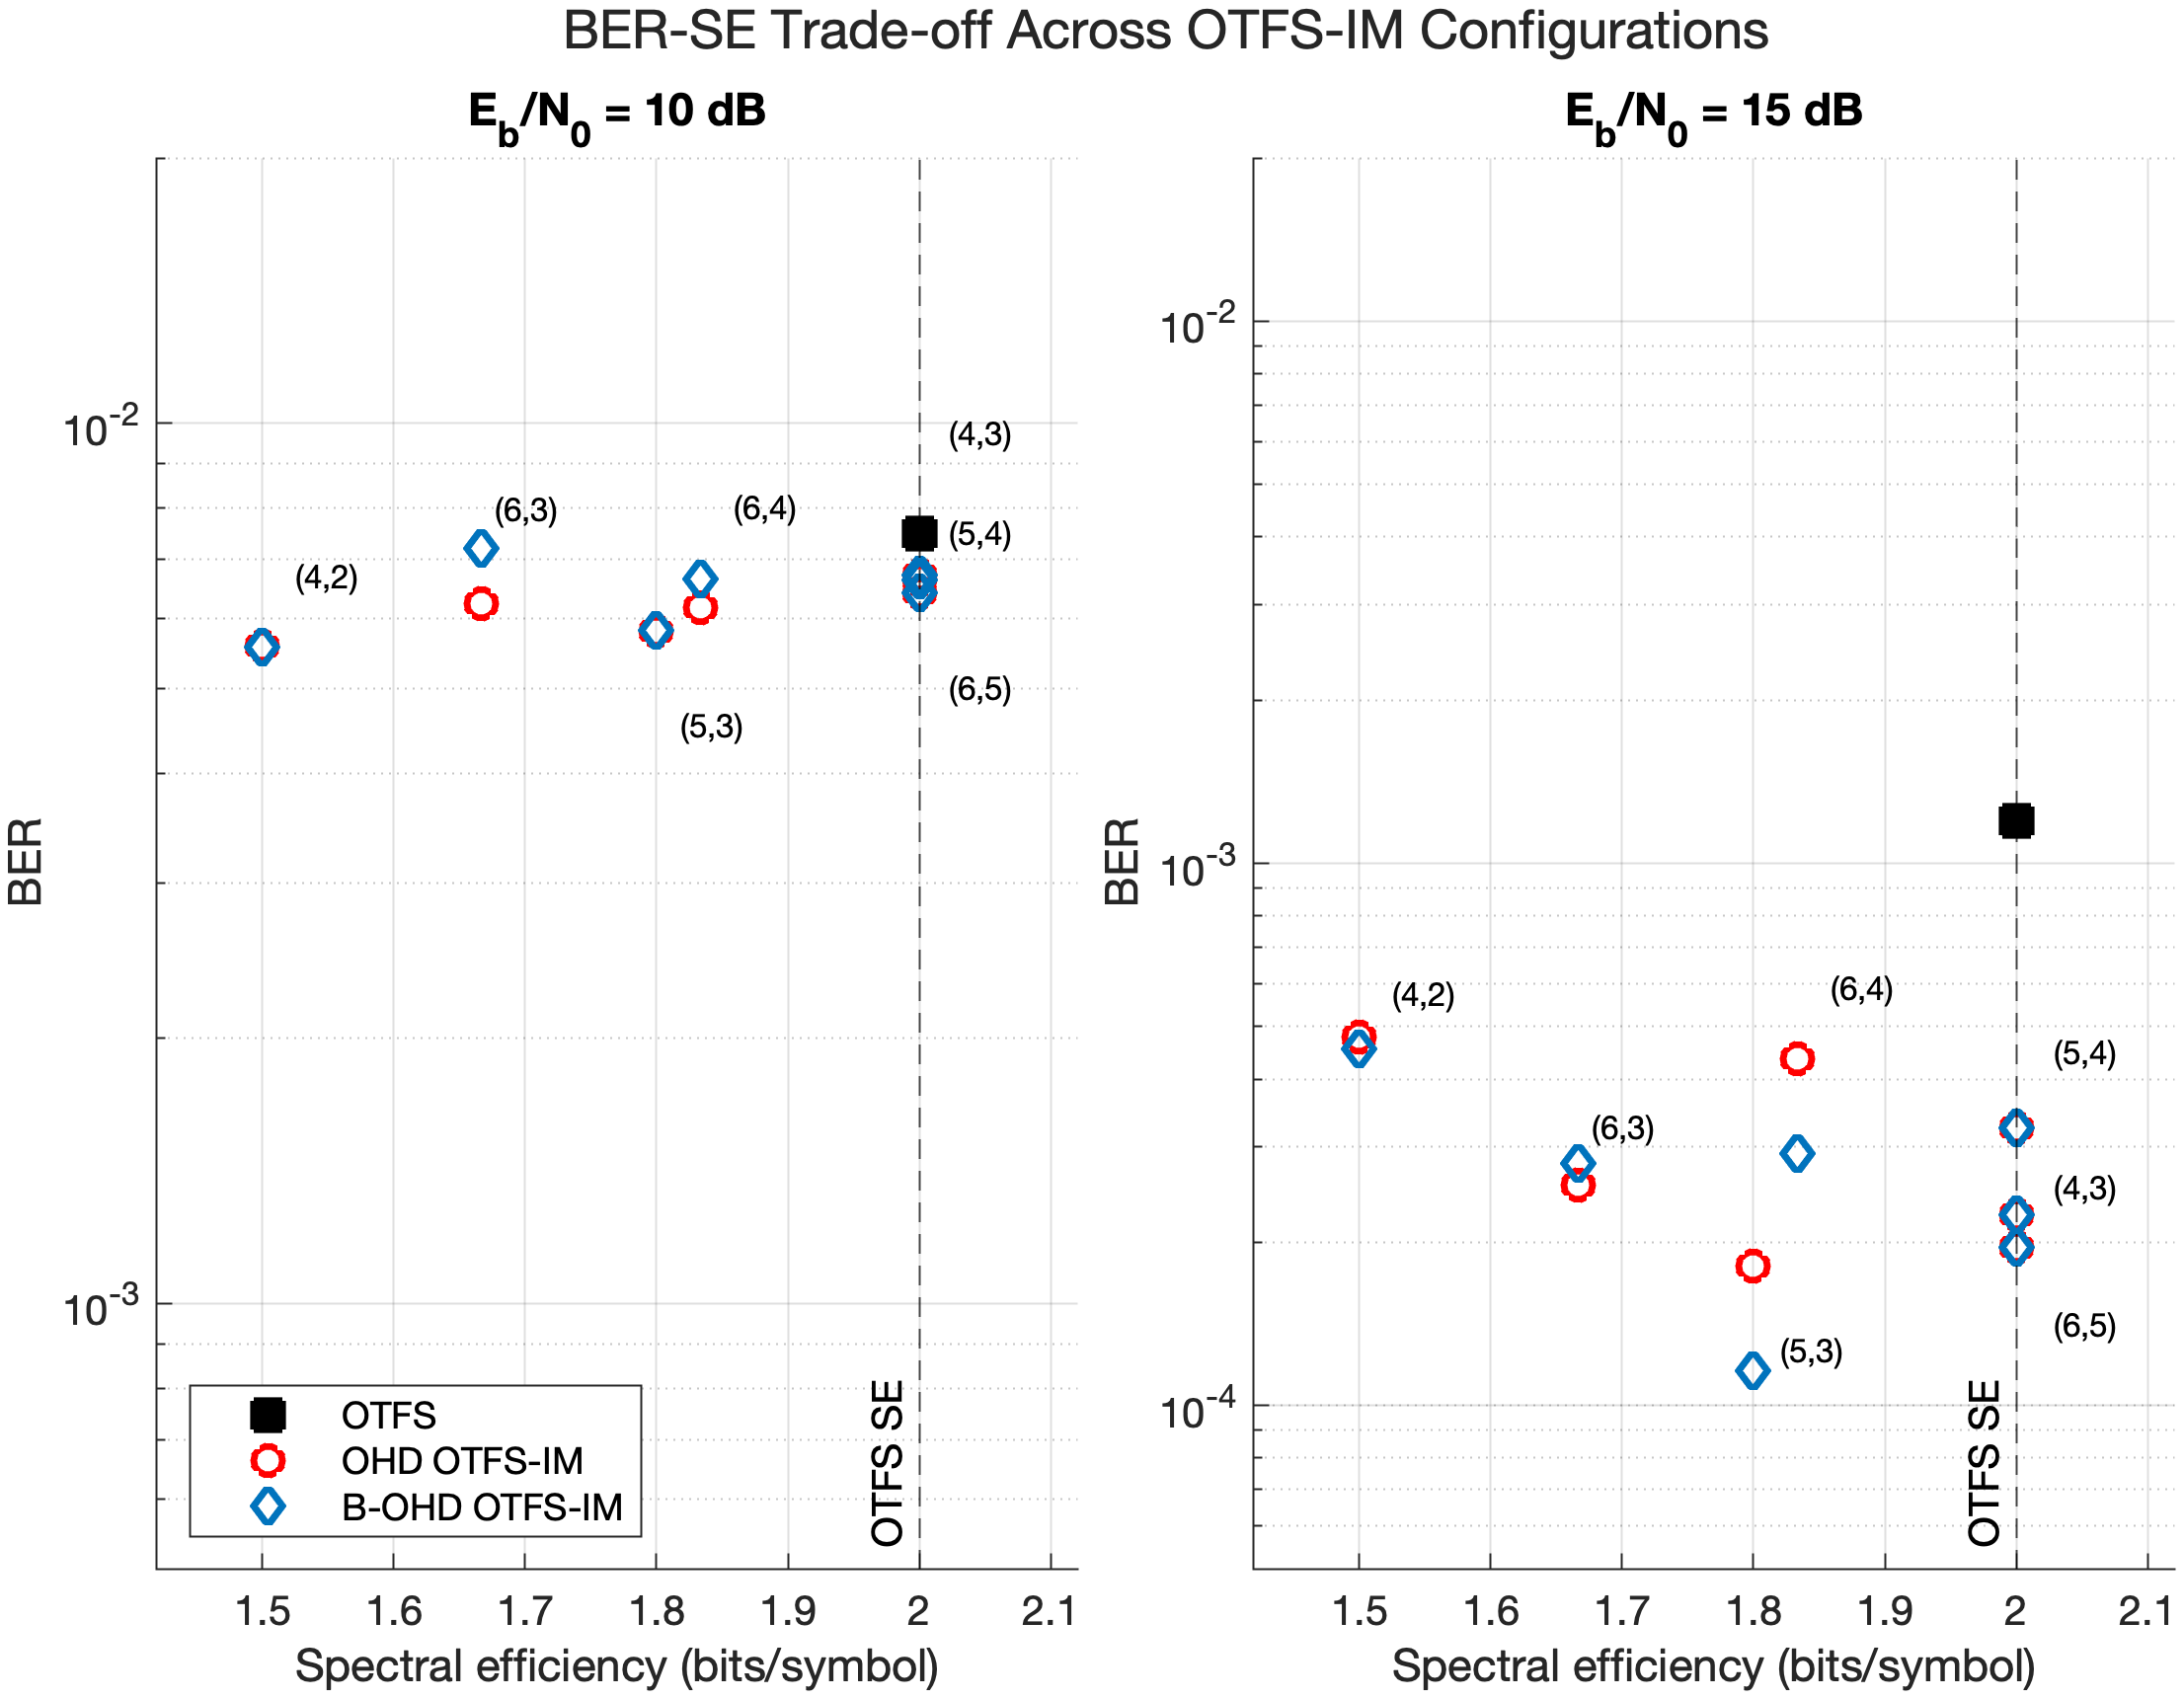
\includegraphics[width=0.95\linewidth]{Images/Chapter5/ber_se_tradeoff.png}
    \caption{BER-SE trade-off across OTFS-IM configurations at selected SNR points}
    \label{fig:chapter5_ber_se_tradeoff}
\end{figure}
}{%
\begin{figure}[H]
    \centering
    \fbox{%
        \begin{minipage}[c][0.28\textheight][c]{0.88\linewidth}
            \centering
            Required figure file is missing:\\
            Images/Chapter5/ber\_se\_tradeoff.png
        \end{minipage}
    }
    \caption{BER-SE trade-off across OTFS-IM configurations at selected SNR points}
    \label{fig:chapter5_ber_se_tradeoff}
\end{figure}
}

Figure~\ref{fig:chapter5_ber_se_tradeoff} gives a more complete interpretation of the same results. The vertical dashed line marks the spectral efficiency of the baseline OTFS system, which is \(2.00~\text{bits/symbol}\) for 4-QAM. Points located on this line correspond to equal-SE OTFS-IM configurations, while points to the left correspond to lower-SE configurations. This representation is important because a lower BER at a smaller spectral efficiency should not be interpreted in the same way as a lower BER at equal spectral efficiency.

The equal-SE configurations, including \(n=4,k=3\), \(n=5,k=4\), and \(n=6,k=5\), are the most direct comparison against baseline OTFS. These cases show that OTFS-IM can preserve the same nominal spectral efficiency while improving BER in the simulated delay-Doppler channel. Among them, the \(n=6,k=5\) configuration is the main equal-SE example used in this chapter because it has a larger IM block and provides clearer high-SNR performance separation from baseline OTFS. However, the overlap between OHD and B-OHD in this case also shows that the proposed balancing criterion does not always change the selected pattern table.

The lower-SE configurations, such as \(n=4,k=2\), \(n=5,k=3\), \(n=6,k=3\), and \(n=6,k=4\), occupy the left side of the trade-off plot. Their BER values are generally competitive because they transmit fewer information bits per block. These configurations are useful when reliability is prioritized over throughput, but their gains must be described as BER-SE trade-offs rather than pure improvements over baseline OTFS. In particular, the \(n=5,k=3\) case is valuable because it demonstrates the difference between OHD and B-OHD in a setting where exact pattern selection remains feasible and the pattern table is not trivially identical.

The comparison also shows that B-OHD should be interpreted as a refinement of OHD rather than a universally dominant detector or modulation method. B-OHD does not change the OTFS-IM signal model, the MP detector, or the modulation order. It only changes the selected activation-pattern table by adding a carrier-usage balancing criterion. Therefore, its gain appears mainly when the selected table has room for improvement in usage balance and when the detector output is reliable enough for such pattern-level differences to affect the final decision.

Overall, the BER-SE summary supports three design insights. First, OTFS-IM can outperform baseline OTFS in the simulated high-Doppler delay-Doppler channel, especially from the medium-SNR region onward. Second, equal-SE configurations are the strongest evidence that OTFS-IM is not merely improving BER by lowering the information rate. Third, pattern selection remains configuration-dependent: B-OHD can improve OHD when the OHD table is unbalanced, but random or structurally similar tables can sometimes perform competitively. For this reason, the final evaluation should report both the absolute BER curves and the BER-SE trade-off, rather than relying on a single BER plot.


% !TEX root = ../../main.tex

\subsection{Design Insights and Chapter Summary}

This chapter evaluated the baseline OFDM-LMMSE, baseline OTFS, and OTFS-IM systems under the same delay-Doppler channel and modulation assumptions. The results show that OTFS-IM is not simply an additional mapping layer placed on top of OTFS. Its performance depends jointly on the IM block size, the number of active positions, the spectral efficiency, the selected activation-pattern table, and the reliability of the detector output. Therefore, the most meaningful conclusion is obtained by reading the BER curves together with the error-decomposition and BER-SE trade-off results.

The first important observation is that OTFS-IM can improve BER over baseline OTFS in the simulated high-Doppler delay-Doppler channel. This is most clearly shown in the medium-to-high-SNR region, where the detector output becomes reliable enough for the activation pattern and symbol decisions to separate more cleanly. In the equal-spectral-efficiency cases, especially \(n=6,k=5\), OTFS-IM preserves the same nominal rate as baseline OTFS while reducing BER. This is the strongest result in the chapter because it shows that the gain does not only come from lowering the number of transmitted information bits.

At low SNR, the advantage of OTFS-IM is less consistent. In this region, the received samples are strongly affected by noise, and the MP detector has difficulty distinguishing both the active positions and the transmitted QAM symbols. As a result, the total BER is influenced more by detector uncertainty than by the exact geometry of the selected pattern table. This explains why OHD, B-OHD, and random selection can be close to each other at some SNR points. It also explains why pattern selection alone cannot be expected to solve all low-SNR errors.

The error-decomposition results provide a more detailed view of the OTFS-IM error mechanism. The total BER is produced by two different sources: index-bit errors and symbol-bit errors. Index errors occur when the receiver selects the wrong active-position pattern, while symbol errors occur when the active positions are detected but the QAM symbols are decoded incorrectly. In the simulated results, symbol errors remain a major contribution to the total BER, especially at moderate SNR. This means that improving pattern geometry is useful, but it should be combined with reliable detection and symbol estimation. A pattern table with good Hamming-distance properties cannot fully compensate for poor detector reliability.

The comparison between OHD and B-OHD gives a more careful interpretation of the proposed pattern-selection improvement. OHD selects activation patterns by prioritizing Hamming-distance separation. B-OHD keeps this idea but additionally considers carrier-usage balance. This makes B-OHD a refinement of OHD rather than a different receiver or a different modulation scheme. The gain of B-OHD appears when the OHD table is unbalanced and when the selected table can be modified without reducing the minimum Hamming distance. The \(n=5,k=3\) configuration illustrates this behavior because B-OHD improves the usage distribution and provides better performance than OHD at the selected operating points.

However, B-OHD does not always produce a different pattern table. In configurations such as \(n=6,k=5\), the selected OHD and B-OHD tables can become effectively identical, leading to overlapping BER curves. This is not a simulation error. It means that the OHD solution is already balanced enough under that configuration, or that the available candidate patterns do not allow B-OHD to produce a meaningfully different table. This result is useful because it prevents an overclaimed conclusion: B-OHD is beneficial when the pattern-selection problem has room for balancing, but it is not universally superior in every \((n,k)\) setting.

The random-pattern baseline also plays an important role in the evaluation. It shows whether a deterministic pattern-selection rule is truly useful or whether similar performance could be obtained from an arbitrary pattern table. In some cases, the random average is competitive with OHD or B-OHD, particularly when the number of candidate patterns is small or when several pattern tables have similar distance properties. Therefore, the random baseline should not be removed from the analysis. Its presence makes the evaluation more honest and strengthens the conclusion that pattern selection is configuration-dependent.

The BER-SE trade-off analysis further clarifies how the configurations should be interpreted. Equal-SE configurations such as \(n=4,k=3\), \(n=5,k=4\), and \(n=6,k=5\) provide the fairest direct comparison with baseline OTFS because they preserve the same spectral efficiency of \(2.00~\text{bits/symbol}\). Lower-SE configurations, such as \(n=4,k=2\), \(n=5,k=3\), \(n=6,k=3\), and \(n=6,k=4\), may achieve lower BER, but part of that improvement comes from transmitting fewer information bits per IM block. These lower-SE configurations are still useful because practical communication systems may choose reliability over rate in difficult channel conditions, but their results should be described as a rate-reliability trade-off rather than a strict performance gain at equal rate.

From a design perspective, the simulation results suggest that the choice of \((n,k)\) should not be made only from the spectral-efficiency formula. A larger \(k\) can help preserve rate, while a smaller \(k\) may improve reliability by reducing the number of active symbols and changing the pattern-detection problem. At the same time, increasing \(n\) enlarges the pattern space and can make exact pattern selection more expensive. Therefore, the final OTFS-IM design must balance spectral efficiency, BER performance, pattern-selection complexity, and detector reliability.

The results also reveal several limitations of the present simulation framework. First, the channel is modeled in the delay-Doppler domain with discrete delay and Doppler taps, but the simulation does not sweep a physical velocity parameter. Therefore, the results support the evaluation of a high-Doppler or doubly selective channel model, while a separate velocity-based study would be needed to quantify performance at specific speeds such as vehicular, railway, or UAV scenarios. Second, the Monte Carlo simulation uses a finite number of frames, so very low BER points may still contain statistical variation. Third, the receiver uses the same general MP detection principle for the compared OTFS-IM designs; more advanced channel-aware, detector-aware, or soft-output detection methods may further change the relative performance.

In summary, this chapter confirms that OTFS-IM is a meaningful extension of baseline OTFS for delay-Doppler-domain transmission. The simulations show that OTFS-IM can improve BER, including in equal-SE cases, and that pattern-table design affects the reliability of index detection. The proposed B-OHD method improves OHD when carrier-usage balancing changes the selected pattern table, but its gain is configuration-dependent. These findings provide the basis for the final conclusion of the thesis: OTFS-IM offers a flexible BER-SE design space for high-mobility-oriented wireless channels, and structured pattern selection is a useful but not standalone component of that design.


\newpage
